
%% bare_conf.tex
%% V1.4a
%% 2014/09/17
%% by Michael Shell
%% See:
%% http://www.michaelshell.org/
%% for current contact information.
%%
%% This is a skeleton file demonstrating the use of IEEEtran.cls
%% (requires IEEEtran.cls version 1.8a or later) with an IEEE
%% conference paper.
%%
%% Support sites:
%% http://www.michaelshell.org/tex/ieeetran/
%% http://www.ctan.org/tex-archive/macros/latex/contrib/IEEEtran/
%% and
%% http://www.ieee.org/

%%*************************************************************************
%% Legal Notice:
%% This code is offered as-is without any warranty either expressed or
%% implied; without even the implied warranty of MERCHANTABILITY or
%% FITNESS FOR A PARTICULAR PURPOSE! 
%% User assumes all risk.
%% In no event shall IEEE or any contributor to this code be liable for
%% any damages or losses, including, but not limited to, incidental,
%% consequential, or any other damages, resulting from the use or misuse
%% of any information contained here.
%%
%% All comments are the opinions of their respective authors and are not
%% necessarily endorsed by the IEEE.
%%
%% This work is distributed under the LaTeX Project Public License (LPPL)
%% ( http://www.latex-project.org/ ) version 1.3, and may be freely used,
%% distributed and modified. A copy of the LPPL, version 1.3, is included
%% in the base LaTeX documentation of all distributions of LaTeX released
%% 2003/12/01 or later.
%% Retain all contribution notices and credits.
%% ** Modified files should be clearly indicated as such, including  **
%% ** renaming them and changing author support contact information. **
%%
%% File list of work: IEEEtran.cls, IEEEtran_HOWTO.pdf, bare_adv.tex,
%%                    bare_conf.tex, bare_jrnl.tex, bare_conf_compsoc.tex,
%%                    bare_jrnl_compsoc.tex, bare_jrnl_transmag.tex
%%*************************************************************************


% *** Authors should verify (and, if needed, correct) their LaTeX system  ***
% *** with the testflow diagnostic prior to trusting their LaTeX platform ***
% *** with production work. IEEE's font choices and paper sizes can       ***
% *** trigger bugs that do not appear when using other class files.       ***                          ***
% The testflow support page is at:
% http://www.michaelshell.org/tex/testflow/



\documentclass[conference]{IEEEtran}
% Some Computer Society conferences also require the compsoc mode option,
% but others use the standard conference format.
%
% If IEEEtran.cls has not been installed into the LaTeX system files,
% manually specify the path to it like:
% \documentclass[conference]{../sty/IEEEtran}





% Some very useful LaTeX packages include:
% (uncomment the ones you want to load)


% *** MISC UTILITY PACKAGES ***
%
%\usepackage{ifpdf}
% Heiko Oberdiek's ifpdf.sty is very useful if you need conditional
% compilation based on whether the output is pdf or dvi.
% usage:
% \ifpdf
%   % pdf code
% \else
%   % dvi code
% \fi
% The latest version of ifpdf.sty can be obtained from:
% http://www.ctan.org/tex-archive/macros/latex/contrib/oberdiek/
% Also, note that IEEEtran.cls V1.7 and later provides a builtin
% \ifCLASSINFOpdf conditional that works the same way.
% When switching from latex to pdflatex and vice-versa, the compiler may
% have to be run twice to clear warning/error messages.






% *** CITATION PACKAGES ***
%
%\usepackage{cite}
% cite.sty was written by Donald Arseneau
% V1.6 and later of IEEEtran pre-defines the format of the cite.sty package
% \cite{} output to follow that of IEEE. Loading the cite package will
% result in citation numbers being automatically sorted and properly
% "compressed/ranged". e.g., [1], [9], [2], [7], [5], [6] without using
% cite.sty will become [1], [2], [5]--[7], [9] using cite.sty. cite.sty's
% \cite will automatically add leading space, if needed. Use cite.sty's
% noadjust option (cite.sty V3.8 and later) if you want to turn this off
% such as if a citation ever needs to be enclosed in parenthesis.
% cite.sty is already installed on most LaTeX systems. Be sure and use
% version 5.0 (2009-03-20) and later if using hyperref.sty.
% The latest version can be obtained at:
% http://www.ctan.org/tex-archive/macros/latex/contrib/cite/
% The documentation is contained in the cite.sty file itself.






% *** GRAPHICS RELATED PACKAGES ***
%
\ifCLASSINFOpdf
   \usepackage[pdftex]{graphicx}
  % declare the path(s) where your graphic files are
  % \graphicspath{{../pdf/}{../jpeg/}}
  % and their extensions so you won't have to specify these with
  % every instance of \includegraphics
  % \DeclareGraphicsExtensions{.pdf,.jpeg,.png}
\else
  % or other class option (dvipsone, dvipdf, if not using dvips). graphicx
  % will default to the driver specified in the system graphics.cfg if no
  % driver is specified.
  % \usepackage[dvips]{graphicx}
  % declare the path(s) where your graphic files are
  % \graphicspath{{../eps/}}
  % and their extensions so you won't have to specify these with
  % every instance of \includegraphics
  % \DeclareGraphicsExtensions{.eps}
\fi
% graphicx was written by David Carlisle and Sebastian Rahtz. It is
% required if you want graphics, photos, etc. graphicx.sty is already
% installed on most LaTeX systems. The latest version and documentation
% can be obtained at: 
% http://www.ctan.org/tex-archive/macros/latex/required/graphics/
% Another good source of documentation is "Using Imported Graphics in
% LaTeX2e" by Keith Reckdahl which can be found at:
% http://www.ctan.org/tex-archive/info/epslatex/
%
% latex, and pdflatex in dvi mode, support graphics in encapsulated
% postscript (.eps) format. pdflatex in pdf mode supports graphics
% in .pdf, .jpeg, .png and .mps (metapost) formats. Users should ensure
% that all non-photo figures use a vector format (.eps, .pdf, .mps) and
% not a bitmapped formats (.jpeg, .png). IEEE frowns on bitmapped formats
% which can result in "jaggedy"/blurry rendering of lines and letters as
% well as large increases in file sizes.
%
% You can find documentation about the pdfTeX application at:
% http://www.tug.org/applications/pdftex





% *** MATH PACKAGES ***
%
%\usepackage[cmex10]{amsmath}
% A popular package from the American Mathematical Society that provides
% many useful and powerful commands for dealing with mathematics. If using
% it, be sure to load this package with the cmex10 option to ensure that
% only type 1 fonts will utilized at all point sizes. Without this option,
% it is possible that some math symbols, particularly those within
% footnotes, will be rendered in bitmap form which will result in a
% document that can not be IEEE Xplore compliant!
%
% Also, note that the amsmath package sets \interdisplaylinepenalty to 10000
% thus preventing page breaks from occurring within multiline equations. Use:
%\interdisplaylinepenalty=2500
% after loading amsmath to restore such page breaks as IEEEtran.cls normally
% does. amsmath.sty is already installed on most LaTeX systems. The latest
% version and documentation can be obtained at:
% http://www.ctan.org/tex-archive/macros/latex/required/amslatex/math/





% *** SPECIALIZED LIST PACKAGES ***
%
%\usepackage{algorithmic}
% algorithmic.sty was written by Peter Williams and Rogerio Brito.
% This package provides an algorithmic environment fo describing algorithms.
% You can use the algorithmic environment in-text or within a figure
% environment to provide for a floating algorithm. Do NOT use the algorithm
% floating environment provided by algorithm.sty (by the same authors) or
% algorithm2e.sty (by Christophe Fiorio) as IEEE does not use dedicated
% algorithm float types and packages that provide these will not provide
% correct IEEE style captions. The latest version and documentation of
% algorithmic.sty can be obtained at:
% http://www.ctan.org/tex-archive/macros/latex/contrib/algorithms/
% There is also a support site at:
% http://algorithms.berlios.de/index.html
% Also of interest may be the (relatively newer and more customizable)
% algorithmicx.sty package by Szasz Janos:
% http://www.ctan.org/tex-archive/macros/latex/contrib/algorithmicx/




% *** ALIGNMENT PACKAGES ***
%
%\usepackage{array}
% Frank Mittelbach's and David Carlisle's array.sty patches and improves
% the standard LaTeX2e array and tabular environments to provide better
% appearance and additional user controls. As the default LaTeX2e table
% generation code is lacking to the point of almost being broken with
% respect to the quality of the end results, all users are strongly
% advised to use an enhanced (at the very least that provided by array.sty)
% set of table tools. array.sty is already installed on most systems. The
% latest version and documentation can be obtained at:
% http://www.ctan.org/tex-archive/macros/latex/required/tools/


% IEEEtran contains the IEEEeqnarray family of commands that can be used to
% generate multiline equations as well as matrices, tables, etc., of high
% quality.




% *** SUBFIGURE PACKAGES ***
%\ifCLASSOPTIONcompsoc
%  \usepackage[caption=false,font=normalsize,labelfont=sf,textfont=sf]{subfig}
%\else
%  \usepackage[caption=false,font=footnotesize]{subfig}
%\fi
% subfig.sty, written by Steven Douglas Cochran, is the modern replacement
% for subfigure.sty, the latter of which is no longer maintained and is
% incompatible with some LaTeX packages including fixltx2e. However,
% subfig.sty requires and automatically loads Axel Sommerfeldt's caption.sty
% which will override IEEEtran.cls' handling of captions and this will result
% in non-IEEE style figure/table captions. To prevent this problem, be sure
% and invoke subfig.sty's "caption=false" package option (available since
% subfig.sty version 1.3, 2005/06/28) as this is will preserve IEEEtran.cls
% handling of captions.
% Note that the Computer Society format requires a larger sans serif font
% than the serif footnote size font used in traditional IEEE formatting
% and thus the need to invoke different subfig.sty package options depending
% on whether compsoc mode has been enabled.
%
% The latest version and documentation of subfig.sty can be obtained at:
% http://www.ctan.org/tex-archive/macros/latex/contrib/subfig/




% *** FLOAT PACKAGES ***
%
%\usepackage{fixltx2e}
% fixltx2e, the successor to the earlier fix2col.sty, was written by
% Frank Mittelbach and David Carlisle. This package corrects a few problems
% in the LaTeX2e kernel, the most notable of which is that in current
% LaTeX2e releases, the ordering of single and double column floats is not
% guaranteed to be preserved. Thus, an unpatched LaTeX2e can allow a
% single column figure to be placed prior to an earlier double column
% figure. The latest version and documentation can be found at:
% http://www.ctan.org/tex-archive/macros/latex/base/


%\usepackage{stfloats}
% stfloats.sty was written by Sigitas Tolusis. This package gives LaTeX2e
% the ability to do double column floats at the bottom of the page as well
% as the top. (e.g., "\begin{figure*}[!b]" is not normally possible in
% LaTeX2e). It also provides a command:
%\fnbelowfloat
% to enable the placement of footnotes below bottom floats (the standard
% LaTeX2e kernel puts them above bottom floats). This is an invasive package
% which rewrites many portions of the LaTeX2e float routines. It may not work
% with other packages that modify the LaTeX2e float routines. The latest
% version and documentation can be obtained at:
% http://www.ctan.org/tex-archive/macros/latex/contrib/sttools/
% Do not use the stfloats baselinefloat ability as IEEE does not allow
% \baselineskip to stretch. Authors submitting work to the IEEE should note
% that IEEE rarely uses double column equations and that authors should try
% to avoid such use. Do not be tempted to use the cuted.sty or midfloat.sty
% packages (also by Sigitas Tolusis) as IEEE does not format its papers in
% such ways.
% Do not attempt to use stfloats with fixltx2e as they are incompatible.
% Instead, use Morten Hogholm'a dblfloatfix which combines the features
% of both fixltx2e and stfloats:
%
% \usepackage{dblfloatfix}
% The latest version can be found at:
% http://www.ctan.org/tex-archive/macros/latex/contrib/dblfloatfix/




% *** PDF, URL AND HYPERLINK PACKAGES ***
%
\usepackage{url}
% url.sty was written by Donald Arseneau. It provides better support for
% handling and breaking URLs. url.sty is already installed on most LaTeX
% systems. The latest version and documentation can be obtained at:
% http://www.ctan.org/tex-archive/macros/latex/contrib/url/
% Basically, \url{my_url_here}.




% *** Do not adjust lengths that control margins, column widths, etc. ***
% *** Do not use packages that alter fonts (such as pslatex).         ***
% There should be no need to do such things with IEEEtran.cls V1.6 and later.
% (Unless specifically asked to do so by the journal or conference you plan
% to submit to, of course. )


% correct bad hyphenation here
\hyphenation{op-tical net-works semi-conduc-tor}


\begin{document}
%
% paper title
% Titles are generally capitalized except for words such as a, an, and, as,
% at, but, by, for, in, nor, of, on, or, the, to and up, which are usually
% not capitalized unless they are the first or last word of the title.
% Linebreaks \\ can be used within to get better formatting as desired.
% Do not put math or special symbols in the title.
\title{Dependable Cloud Computing with OpenStack}


% author names and affiliations
% use a multiple column layout for up to three different
% affiliations
\author{\IEEEauthorblockN{Johannes Eschrig}
\IEEEauthorblockA{Hasso Plattner Institute Potsdam\\
Potsdam, Germany\\
Email: johannes.eschrig@student.hpi.de}

\and

\IEEEauthorblockN{Sven Knebel}
\IEEEauthorblockA{Hasso Plattner Institute Potsdam\\
Potsdam, Germany\\
Email: sven.knebel@student.hpi.de}

\and

\IEEEauthorblockN{Nicco Kunzmann}
\IEEEauthorblockA{Hasso Plattner Institute Potsdam\\
Potsdam, Germany\\
Email: nicco.kunzmann@student.hpi.de}}

% conference papers do not typically use \thanks and this command
% is locked out in conference mode. If really needed, such as for
% the acknowledgment of grants, issue a \IEEEoverridecommandlockouts
% after \documentclass

% for over three affiliations, or if they all won't fit within the width
% of the page, use this alternative format:
% 
%\author{\IEEEauthorblockN{Michael Shell\IEEEauthorrefmark{1},
%Homer Simpson\IEEEauthorrefmark{2},
%James Kirk\IEEEauthorrefmark{3}, 
%Montgomery Scott\IEEEauthorrefmark{3} and
%Eldon Tyrell\IEEEauthorrefmark{4}}
%\IEEEauthorblockA{\IEEEauthorrefmark{1}School of Electrical and Computer Engineering\\
%Georgia Institute of Technology,
%Atlanta, Georgia 30332--0250\\ Email: see http://www.michaelshell.org/contact.html}
%\IEEEauthorblockA{\IEEEauthorrefmark{2}Twentieth Century Fox, Springfield, USA\\
%Email: homer@thesimpsons.com}
%\IEEEauthorblockA{\IEEEauthorrefmark{3}Starfleet Academy, San Francisco, California 96678-2391\\
%Telephone: (800) 555--1212, Fax: (888) 555--1212}
%\IEEEauthorblockA{\IEEEauthorrefmark{4}Tyrell Inc., 123 Replicant Street, Los Angeles, California 90210--4321}}




% use for special paper notices
%\IEEEspecialpapernotice{(Invited Paper)}




% make the title area
\maketitle

% As a general rule, do not put math, special symbols or citations
% in the abstract
\begin{abstract}
Offering infrastructures as a service by means of cloud computing is gaining popularity. High availability aspects of these cloud computing systems are of great importance, as outages can be extremely costly. Setting up a cloud computing environment is very complex, thus making dependability testing non trivial. In our work, we introduce a system for installing a virtual OpenStack cloud computing environment and running dependability experiments on it\footnote{\url{https://github.com/MasterprojectOpenStack2015/sourcecode}}. The installation as well as the experiments are automated in order to achieve reproducible test results as easily as possible. We propose a first selection of experiments for our testing framework and describe the results.
\end{abstract}

% no keywords




% For peer review papers, you can put extra information on the cover
% page as needed:
% \ifCLASSOPTIONpeerreview
% \begin{center} \bfseries EDICS Category: 3-BBND \end{center}
% \fi
%
% For peerreview papers, this IEEEtran command inserts a page break and
% creates the second title. It will be ignored for other modes.
\IEEEpeerreviewmaketitle



\section{Introduction}
% no \IEEEPARstart
As cloud computing becomes more and more popular, there are an increasing number of  implementations to offer various cloud-service models like infrastructure as a service (IaaS), platform as a service (PaaS) or software as a service (SaaS). While many companies offer commercial solutions like the Amazon Elastic Compute Cloud (EC2) or HP Helion, there are also open source alternatives that can be freely installed and configured to meet the needs of ones projects with respect to the underlying hardware available.

One of the open source variants for achieving a cloud computing system is OpenStack. OpenStack is a cloud software stack which allows for offering infrastructure as a service, almost independent of the underlying hardware setup. OpenStack itself can be seen as a collection of services that can be setup depending on the specifications of the planned use cases. The most important components that OpenStack offers are the networking, virtualization and storage services. Furthermore, it is possible to add further components to an OpenStack installation, e.g., services that handle billing or allow for object storage in the cloud. 

This paper will describe the results of the masters project ``Dependable Cloud Computing with OpenStack'' of the summer term 2015 at the Hasso Plattner Institute Potsdam. An important factor, especially in cloud computing, is dependability. When offering such a service, it should be highly available, meaning that the system should be continuously operational without failing. Therefore, our main task was to analyse dependability mechanisms of OpenStack. To do this, we chose to manually setup a clean OpenStack environment (i.e. none provided by a third party like HP Helion) on which we would be able to run the specific analyses. We turned this manual installation into an automated one in order to simplify and speed up the process of setting up a working OpenStack test environment and making the resulting analyses of dependability reproducible. Since no OpenStack installation is exactly the same, the reproducibility of the results of such analyses is not an easy feat. We tackle this issue by making the test environment for the experiments completely virtual. Thus we circumvent tedious hardware setup, hardware errors that disturb the experiments. This also allows an fast rerun of the experiments and switching off network infrastructure. 

\section{Related Work}
\label{related}
In this chapter we will introduce work related to our masters project. In a first part we will describe work related to OpenStack and its possibilities of installation. The second part will cover the related work to dependability in OpenStack.

\subsection{OpenStack Installation}
In order to analyse the dependability of OpenStack, it is necessary to install an OpenStack instance. Due to the fact that such an analysis might require a clean and fresh OpenStack installation after each test run, a quick installation is of advantage. Further, independence of underlying hardware is vital to reproduce results. Merging the requirements of an easy and quick installation that achieve reproducible results leads us to look for possibilities to automatically install OpenStack completely in a virtual environment. There are various OpenStack derivatives both commercially and freely available.

\emph{HP Helion}\footnote{\url{http://www8.hp.com/us/en/cloud/hphelion-openstack.html}} is available both as a commercial-grade edition and a free-to-license community edition. The latter is available on promotional USB drives given out by HP. The HP Helion community edition installation is made to provide an easy installation routine with little need for configuration by means of such an USB drive. Further, it is possible to install HP Helion as an all-in-one system on virtual machines in addition to deploying it on bare-metal. 

\emph{DevStack}\footnote{\url{http://docs.openstack.org/developer/devstack/}} is another possibility for an easy OpenStack installation. It is a development environment for OpenStack. Being designed for development on OpenStack, it is mainly used for an one-node installation of OpenStack. Additionally, DevStack also offers an option for a multi-node setup.

A manual installation of an OpenStack instance can take very long and be quite cumbersome, depending on the setup one is aiming to achieve. It is therefore of great advantage to automate the installation. As an OpenStack installation is distributed among a number of nodes, using an orchestration tool like Ansible\footnote{\url{http://www.ansible.com/}} is advisable. Ansible manages nodes using SSH and Python. 

\emph{openstack-ansible}\footnote{\url{https://github.com/openstack-ansible/openstack-ansible}} is an existing automated OpenStack installation project, which installs OpenStack on Vagrant virtual machines. We ran the installation script of this project, however encountered some bugs. In order to understand the underlying mechanisms of OpenStack ourselves, we decided to follow a similar approach to openstack-ansible based on KVM virtual machines.


\subsection{Evaluating OpenStack Dependability}

Due to the complexity and variety of possibilities to set up an OpenStack system, evaluating the dependability of OpenStack in general is no easy task. For this reason, we have decided to make simplifying assumptions about an OpenStack installation and define a test environment on which we can then run dependability experiments. An more general approach is also possible, i.e. building a framework for injecting faults into various OpenStack deployments, as was done for example by \cite{kollarova} or \cite{Ju:2013:FRO:2523616.2523622}. Both works thereby created a frameworks for injecting faults into OpenStack. \cite{kollarova} follows a similar approach to that of our masters project and uses a virtual environment for the setup of OpenStack, however only implements one simulated failure as proof of concept. \cite{Ju:2013:FRO:2523616.2523622} on the other hand focuses more on the fault injection aspect, especially targeting service communications, uncovering 23 bugs in two OpenStack versions. In our masters project, we aim to provide a framework for the evaluation of the cloud system OpenStack with the advantage of a fast and easy virtual installation of the system itself and easily extendable experiments for dependability testing.

The previous masters project on OpenStack also gave some insights on fault tolerance of OpenStack in \cite{mp14}, presenting a fault tree based on the high availability setup presented by \cite{teng}.


\section{OpenStack Test Environment}
As described in Chapter~\ref{related}, we tried various possibilities to install an OpenStack system on a virtual environment. In this chapter we outline the challenges we faced with these possibilities, ultimately leading to the decision to create our own installation routine for a virtual OpenStack environment. Also, we will describe this test environment in detail.

\subsection{Existing OpenStack Installation Possibilities}
\label{installpossibilities}
We first tried installing the cloud computing environment HP Helion community edition. It promises an easy installation routine with little need for configuration. Further, it is possible to install HP Helion as an all-in-one system on virtual machines in addition to deploying it on bare-metal. This is an advantage with respect to our requirement of achieving a virtual test environment for reproducible test results. However, even though HP Helion has its advantages for setting up one's own IaaS system for a real use scenario, we came to the conclusion that it is not suitable for our needs. The installation of HP Helion took around 90 minutes on our hardware, which is not feasible for repeated installations. Further, we found that HP Helion does not survive a reboot of the host or the virtual machines it is running on. Fixing this issue would have required understanding the underlying installation scripts, which would still not have been beneficial in understanding OpenStack itself. Additionally, with our limited knowledge of HP Helion, it would have been a challenge to customize the system to fit our needs. We thus concluded that we would not use HP Helion for analyzing the dependability of OpenStack in line with this masters project.

A further option for an OpenStack deployment to work with for dependability testing we considered was DevStack. Due to the nature of the use cases for which DevStack is made, multi-node and high-availability setups are not the main focus, and therefore not documented well enough for us to customize DevStack and use it for dependability analyses. Also, it is not possible to generalize results of dependability analyses run on DevStack to a full OpenStack installation, as DevStack is not designed with real deployment in mind. As a result, we decided to use a full OpenStack installation for running our analyses.

\subsection{Specifying our own OpenStack Environment}
\label{environment}
In order to be able to make the OpenStack test environment installation as easy and quick as possible, so that one can concentrate on the dependability analysis, we chose to install OpenStack virtually. A further advantage of this virtual installation is the reproducibility of experiment results, which is important to be able to make scientific statements about the dependability of OpenStack. We used libvirt\footnote{\url{http://libvirt.org/}} to create a number of virtual machines based on simple configuration files and Ansible\footnote{\url{http://www.ansible.com}} to orchestrate the installation of OpenStack on these nodes. The details of this automated installation are described in Chapter~\ref{installing}.

In order to create an useful test environment for dependability experiments, it was necessary to define an architecture. We chose this architecture to be a simplified OpenStack instance, meaning that we focus only the most important of the OpenStack services available. This can be seen as a bottom-up approach, as we focus on evaluating a simpler system than one might encounter when looking at an OpenStack system in production mode. One advantage of this approach is that, due to the simplicity, it is easier to make statements about OpenStack in general, than on one specific system. Libvirt and Ansible allow to add more nodes, create a more complex OpenStack system and, extend the proposed architecture by means of high availability mechanisms. We then draw conclusions about their effectiveness.

Figure~\ref{fig:arch} shows our virtual test environment architecture, which is the proposed architecture of the official OpenStack install guide\footnote{\url{http://docs.openstack.org/kilo/install-guide/install/apt/content/index.html}}. All nodes are virtual machines running on a physical host. The tenant virtual machines are dispatched on the compute node by means of nested virtualization. By default, our environment contains the following nodes:
\begin{itemize}
	\item One controller node: this node runs the OpenStack Dashboard (Horizon), the API services, the MySQL database, the RabbitMQ message queue server, the scheduler for the compute resources, Identity (Keystone) and Image (Glance) services.
	\item One network (Neutron) node: this node handles the internal and external routing and DHCP services for the virtual networks.
	\item Two compute nodes: the compute nodes are the computing resources for running the virtual machines of the OpenStack users. They run the hypervisor and services like \verb|nova-compute|, which is responsible for creating and terminating virtual machine instances through the hypervisor APIs.
	\item Two object storage (Swift) nodes: these nodes operate the OpenStack container and object services and each contain two local block storage disks for persisting the objects.
\end{itemize}

Further, the following networks are used to communicate between nodes and instances:
\begin{itemize}
	\item Management network: this network is used for the OpenStack administration, i.e., it connects the OpenStack services on the different nodes. 
	\item Tenant or tunnel network: these networks can be created by the OpenStack users to achieve communication between projects or instances. 
	\item External network: this network provides internet access to the instances.
\end{itemize}

This architecture is comprehensive enough to test various OpenStack use cases and analyze the dependability of the system.

\begin{figure}[h]
	\centering
		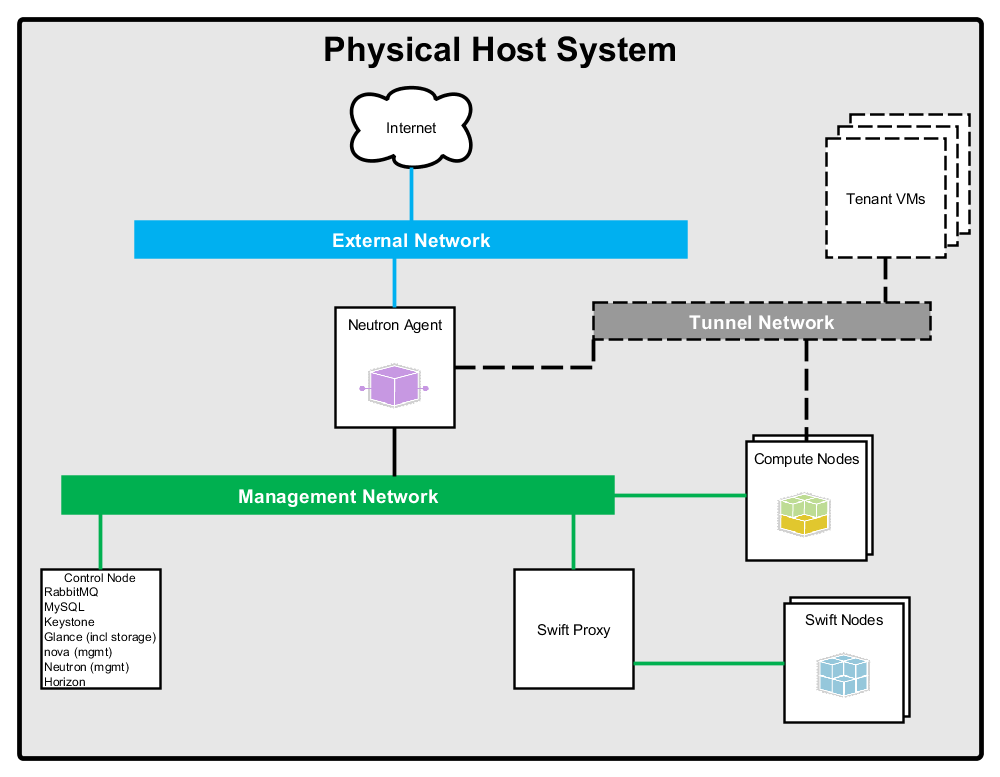
\includegraphics[width=0.50\textwidth]{images/architectureEN.PNG}
	\caption{Our test environment architecture, based on the one proposed by the OpenStack install guide}
	\label{fig:arch}
\end{figure}

The virtual OpenStack installation requires far less hardware resources than a distributed bare metal installation. It is possible to install a fully functional simplified test environment with one compute and object storage node on a quad-core Intel Xeon machine with 8GB RAM. For the full installation, more resources are recommended. We used a 16-core machine with 64GB RAM. 

\section{Automated Installation of OpenStack}
\label{installing}

In this chapter, we describe the automated installation process of OpenStack on our virtual environment. We give an introduction to the usage and a conceptual overview.

\subsection{How to Install OpenStack using our System}
The installation scripts are developed and tested on a Ubunutu 14.04 LTE (Trusty Tahr) desktop version. All required dependencies (e.g., Ansible, libvirt, etc.) are installed automatically, thus an internet connection is required. It installs OpenStack virtually creating the architecture described in Capter~\ref{environment}. The virtual machines are automatically created. The installation takes between 10-15 minutes

After the successful installation, a snapshot named ``initial'' is created. This allows for thorough dependability testing without re-installing the whole system after each experiment. Snapshots can be created manually as well. The snapshotting mechanism will shut down all virtual machines, snapshot the virtual hard drives of all nodes, and bring back up all machines.

\subsection{Creating the Virtual Environment}
\label{subsec:createve}
The virtual environment, i.e., the virtual networks and the virtual machines, are defined in the \verb|config| folder as libvirt network and libvirt domain XML-files. These XML-files define for example the IP addresses of the networks or the hardware specifications (size of RAM, number of cores, virtual hard drives, network interfaces) of the virtual machines. The virtual machines are then created with an Ubuntu cloud image\footnote{\url{https://cloud-images.ubuntu.com/trusty/}}, which are pre-configured images customized especially for running on cloud platforms. 

The initialization of the virtual machines is done using cloud-init\footnote{\url{https://cloudinit.readthedocs.org/}}, which allows for setting passwords and SSH keys for easily connecting to the them afterwards, which is also a prerequisite for utilizing Ansible in the next steps. Further, using cloud-init, the correct \verb|etc/network/interfaces| configuration files are copied to the virtual machines. 

In addition to the virtual machines for the OpenStack nodes, a further virtual machine named ``aptcache'' is created. This machine is used as a package repository by the others. The packages it delivers are not updated, meaning that the versions of all installed packages are frozen. This is important for acquiring a reproducible test environment and prevents different experiment outcomes to be caused by different package versions throughout the system.

These virtual machines create the base of the virtual OpenStack test environment and are now ready for the actual OpenStack installation.

\subsection{Installing OpenStack on Virtual Machines with Ansible}
In order to be able to install OpenStack on the created virtual environment, Ansible must be configured in such a way that virtual machines are grouped. This allows for installing different parts of OpenStack on the different nodes. These groups are defined in a so called Ansible hosts file, which assigns the IP addresses of the different nodes to different groups. In our case, each node type is a group, i.e., ``controller'', ``network'', ``compute'' and ``object''. This allows for the so called Ansible playbooks to be executed on the specified groups of nodes in parallel. 

The Ansible playbooks that run the installation of OpenStack on the virtual nodes are strongly based on the official OpenStack installation guide\footnote{\url{http://docs.openstack.org/kilo/install-guide/install/apt/content/index.html}}, which is very extensive. This gives the advantage of not having to write any further OpenStack related documentation additionally to the documentation of the technicalities of the creation of the virtual machines and the Ansible installation. The arrangement of the Ansible playbooks in a folder structure derived from the content of the OpenStack documentation allows for easily finding the corresponding part of the documentation should one require information about a certain part of the installation.

The Ansible installation of OpenStack starts with an initial preconfiguration of the virtual nodes. In this step, the hosts files are created in order to be able to connect to the nodes by their host names. These host names are then also added to the SSH \verb|known_hosts| files to enable the SSH connection without warning messages. Further steps include setting the locale of the virtual machines to prevent locale errors as well as deactivating the \verb|/etc/cloud/cloud.cfg| file, as all configuration of the images is done in the previous step, see Chapter~\ref{subsec:createve}.

A special virtual machine named ``aptcache'' is set up first and independently of the others. It runs Apt-Cacher-NG\footnote{\url{https://www.unix-ag.uni-kl.de/~bloch/acng/}}, a caching proxy for Linux package repositories. All other VMs are set up to request their packages through it. This a) decreases network traffic and wait times and b) can be used to repeat the setup process while using the exact same package versions as the first time: The first install seeds the package cache, a repeated installation then can receive all packages from the cache instead of fetching potentially newer versions from upstream. To allow this, the cached data is not stored in the VM, but in a folder shared from the host machine.

The first step of the actual OpenStack installation is installing the basic environment. This includes adding the OpenStack package repository to the nodes and installing the MySQL database on the controller and the message queue RabbitMQ on all nodes.

The next step is the installation of the OpenStack identity service (Keystone) on the controller node. This service is responsible for the permissions of users and keeping track of the available OpenStack services with their endpoints. The installation of this service includes creating a database, installing the Keystone client packages and populating the database. A demo and an admin tenant are initially created. As with all OpenStack services, the installation is finalized by creating the service entity and the API endpoint.

Next, the image service Glance is added on the controller node. This service allows for retrieving and registering virtual machine images. Again, a database for this service is created along with the installation of the Glance client packages and the creation of an API endpoint.

OpenStack compute is then setup on the controller and the compute nodes. This component is responsible for the administration and hosting of the computing systems. It allows - among other things - for creating and terminating virtual machine instances through hypervisor APIs and is responsible for scheduling on which compute node an instance should run. To install the compute service Nova on the controller, the respective database and API endpoint is created and the nova service is configured. On the compute nodes, the nova-compute packages are installed and configured to run a QEMU hypervisor with the KVM extension.

The OpenStack networking Neutron components are installed next on the network, controller and compute nodes. The main responsibility of the networking component is to provide connectivity between the instances running on the compute node. On the controller node, database and endpoint API are created, the networking server component is configured and the Modular Layer 2 plug-in is configured. This plug-in is responsible for the networking framework of the instances running on the compute nodes. On the network node, the networking components are installed and configured accordingly. The layer-3 agent for routing services, the DHCP agent, the metadata agent and the Open vSwitch service are configured. Lastly, the networking components, the Modular Layer 2 plug-in and the Open vSwitch service are configured on the compute node. The external and tenant networks are then created to finalize the installation.

The OpenStack web interface dashboard Horizon is then installed on the controller node. This allows administrators and users to access and manage their resources on the OpenStack cloud.

The last component that is added to OpenStack in regards to this masters project is the object storage Swift. This allows to create containers, upload and download files and management of the objects on the storage nodes. On the controller node, the proxy service that handles the requests for the storage nodes is installed and configured. The storage nodes require two empty storage devices for persisting the objects. The virtual machines for these nodes contain two virtual devices in the qcow file format. The OpenStack Swift components are then installed and configured on the object storage nodes. Following the installation, the initial account, container and object rings are created.


\section{Running Dependability Experiments}
\label{experiments}
In this chapter, we will describe our OpenStack dependability experiments and their results. The implementations of these experiments all follow the same structure, so that it is easy to add further experiments if needed. In our experiments, we focused on covering the failure of various OpenStack components or nodes. We will give insights on how these failures affect the OpenStack environment and how the system deals with each fault. This serves partly to show weak points of the setup and partly to document details about its behaviour.

Experiments consist of multiple stages: The \emph{setup} stage creates all elements necessary to run the experiment. The \emph{break} stage then breaks things. An optional \emph{heal} stage tries something simple to undo the damage (e.g. reboot a shutdown node). After each of this stages, a \emph{check} step is executed, which observes the state of the system and reports its findings to the user. Generally, after the setup stage all checks should be successful. Where user observations are useful (e.g. by looking not just at API results, but seeing how Horizon represents situations), the user is prompted to do so.

Using the snapshotting mechanism, the user can always completely restore the system, even if it didn't survive an experiment. This is not done by default because a) it takes some time and is not always necessary and b) to allow the user to inspect the system state after the experiment has concluded, e.g. to find or work out steps to fix remaining issues.

\subsection{Experiment Results}
This section describes our four example experiments and discusses their results. 

\subsubsection{Experiment 1: Control Node crash}
In this experiment, a crash of the control node in the system is simulated. 

\textbf{Technical Background}
The controller node stores global information of the OpenStack cluster and runs the sub-services depending on it, which then give services on other nodes the specific information they need to e.g. run a specific instance or to build network connectivity. In our setup, it also provides the dashboard Horizon and runs the authentication service. A failure of this node obviously is going to have a large impact, but some things that already are set up on other nodes continue to operate.

\textbf{Experiment}
The experiment script creates an instance and then uses ping to verify availability of both the compute node and the started instance. It also tries to access OpenStack APIs. To simulate the fault, it either issues a shutdown command, simulating the unavailability of the node to the controller or more severely, just turns off its infrastructure virtual machine to simulate a full crash.

\textbf{Results and Conclusion}
While the control node is turned off, outside connectivity to the already created instance remains, since it runs on the compute node and its network connection to the outside (managed by Neutron, via the network node) is unaffected. On the other hand, all attempts to use OpenStack APIs fail. Most user-facing APIs are accessed via the controller and thus completely unavailable. Others report errors, since every action has to be authorized using the Keystone service, which only runs on the compute node in our setup.

After the controller node is up again, OpenStack takes a few minutes to re-establish all service connections and in most cases is fully operational again. It is possible that the compute instances fail to reconnect to RabbitMQ and their services have to be restarted manually\footnote{\url{http://docs.openstack.org/openstack-ops/content/maintenance.html\#cloud_controller_storage}}. 

This shows that already running instances on OpenStack are generally not impacted by temporary failure or maintenance of quite a few central OpenStack components, but during their unavailability no changes can be made and recovery might need manual intervention by an operator. 

If the controller node was shut down hard, obviously many more failure scenarios related to the underlying operating system or services are possible, e. g. missing information in databases or damaged file systems.

\subsubsection{Experiment 2: Memchached Service Loss of Data}
This experiment shows the effects of Keystone losing authentication tokens due to the design of its storage mechanism.

\textbf{Technical Background}
A common way to authenticate for operations against the OpenStack API is to use tokens. A more complex and privileged authentication (e.g. a password check) is done once to obtain a security token. These tokens have a limited lifetime and can be limited in scope, so a user can generate a token for a specific task and pass it to a service, which then can use it to access other services in the users name. Tokens also are internal to OpenStack, whereas other authentication might require accessing an external authentication provider (e.g. an LDAP server).

The Keystone service stores these tokens in memcached\footnote{\url{http://memcached.org/}}, which is, as the name alludes to, an in-memory caching service. Designed as just a fast caching layer, it neither has persistence to disk nor does it guarantee to keep all data it stores. If it deems necessary it can evict any information at any time (i.e. because it is under memory pressure).\footnote{\url{https://code.google.com/p/memcached/wiki/NewUserInternals\#How_the_LRU_Decides_What_to_Evict}}

\textbf{Experiment}
The admin credentials are used to create a token. To verify the tokens validity, it is used to authenticate an operation against the Keystone API. To cause memcached to evict it from the cache, the command for memcached to delete all its data is issued. 

\textbf{Results and Conclusion}
Subsequent attempts to use the token fail, since it has been deleted. This shows the consequences of OpenStack using an unreliable data store to save a central element of its authentication system, instead of using memcached as designed only as a cache to improve lookup speeds. 

If a user is  logged into the Horizon dashbord while the experiment is running, it also sometimes allows to observe failures: The dashboard site is still accessible (because the session on the web server still exists), but no information from OpenStack is shown because attempts to retrieve it fail due to the invalid token. The user has to log out and back in again to create a new token. 

\subsubsection{Experiment 3: Compute Nodes Unavailable}
This experiment documents the behaviour if connectivity to compute nodes is lost.

\textbf{Technical Background}
Instances are distributed among the compute nodes by the Nova scheduler, which runs on the controller node. Inspecting the state of VMs, e. g. directly via the Nova API or via the Horizon Dashboard is also done via information stored by Nova on the controller node, where it collects information from all compute hosts.
If the controller looses connectivity to compute nodes, it can't accurately report the state of individual instances, as seen in this experiment. 

\textbf{Experiment}
This experiment first creates an instance to observe throughout the different stages. Then the first level of fault is introduced: All compute nodes are removed from the management network. Then an attempt to start a second instance is made. After this, a more severe fault is created by shutting down all compute nodes. Then a "fix" is attempted by restarting the VMs.

\textbf{Results and Conclusion}
After the first fault,  Nova on the controller has no connectivity to the compute nodes and is therefore unable to actually start the second instance. The first instance is still reported as being active, which in this case is correct: it is still running and can be reached from the outside network. Since it already has lost all connectivity to the compute nodes, things look exactly the same after the compute nodes are actually shut down, but in this case the state information is wrong: the VMs obviously are not active, but shut down together with the host they were running on. After the reboot of the compute nodes, they reconnect to the controller and the state of all VMs is reported correctly again.

This shows that when Nova looses connectivity to a compute node it can't report accurate information, which is one of the reasons why Nova doesn't implement functionality to automatically restart such VMs.  Short interruption of Nova services, e.g. due to software updates, do not necessarily disrupt instance operations. Such decisions are left to other systems that can collect more information (e.g. by running active tests against VMs) and can be configured for specific application needs, like OpenStack Heat. 

We find it interesting that the developers choose to report such instances as active and did not introduce another state to represent this special situation.

%\subsubsection{Experiment 4: Object Storage Crash}
%In this experiment, the crash of object storage (Swift) nodes is simulated. The experiment is setup by uploading a 100 MB test file to the fully functional object storage cluster, consisting of two object storage nodes. 
%
%\textbf{Technical Background}\footnote{Detailed information on OpenStack Swift is given in \cite{swift} or on \url{https://swiftstack.com/openstack-swift/}}
%OpenStack Swift stores the copies of the same data on different nodes to prevent the loss of data in case of failure and to be able to offer massive scalability. As opposed to, e.g., a simple file system, Swift is an eventually consistent storage system. Objects in Swift are stored in containers, which contains meta data about the objects. Containers themselves are contained in an account, which is the storage area. The processes that run on a storage node thus are composed of account, container, object and proxy server processes. The proxy server is responsible for the verification and handling of API requests, as well as for deciding which node to send the request to. This includes choosing a substitute storage node, should the primary one be unavailable. To ensure consistency of the data across the nodes, a Swift auditor service continually checks for malformed data on the disks and moves corrupted objects into a specified quarantine. Replicator services check the hashes of the copies of objects on other nodes, and send out their respective copy of the object should it be inconsistent.
%
%Regarding the architecture of the storage cluster, it can be divided in nodes, regions and zones. Our system runs two storage nodes with one region and zone, as described in the OpenStack documentation we base our system on. Regions represent geographically separated parts of the cluster, and zones separate physical hardware, i.e. different racks. Our storage nodes contain two storage disks each. Swift partitions storage disks into partitions (which in OpenStack indicate rather a directory than a conventional storage partition), the maximum number of which can be configured - in our case $2^{10} = 1024$. These partitions are replicated as uniquely across the cluster as possible a specified number of times. In our system, three replicas are created. The replicas are mapped to the partitions in a hashing ring. 
%
%\textbf{Experiment}
%The experiment contains multiple steps. Aim of the experiment is to verify the availability of a test file download even after the crash of a storage node. Due to the fact that each node has two storage disks, and three replicas of each object are configured, the test file is replicated on one node twice, and on the other once. After the upload of the 100 MB test file, it is downloaded to verify the functionality. Next, a crash of one of the object nodes is simulated. Again, the download is initiated before the node is restarted. This procedure is then done for the simulated crash of the other storage node. In a last step, the crash of both nodes is simulated.
%
%\textbf{Results and Conclusion}
%The results of this experiment show that, for a correctly setup and configured OpenStack system with two storage nodes, a storage node crash will not impair the functionality for the user. The test file object is replicated correctly amongst the nodes, i.e., one node contains two replicas (one on each hard drive), and the other contains one replica. This is due to the fact that Swift tries storing replicas in the most unique way possible amongst the cluster. Only when both storage nodes fail will the download of the test file be impossible. This is an obvious trivial test case that was added to the experiment for completeness.
%
%The number of replicas is crucial for Swift to be able to cope with a storage node crash. Three replicas is a configuration that is found often when applying redundancy to high availability systems. However, two replicas would also suffice for surviving a storage node crash in our setup, as Swift distributes the replicas in the most unique way possible, which would assign both nodes one copy of the test file. 








% An example of a floating figure using the graphicx package.
% Note that \label must occur AFTER (or within) \caption.
% For figures, \caption should occur after the \includegraphics.
% Note that IEEEtran v1.7 and later has special internal code that
% is designed to preserve the operation of \label within \caption
% even when the captionsoff option is in effect. However, because
% of issues like this, it may be the safest practice to put all your
% \label just after \caption rather than within \caption{}.
%
% Reminder: the "draftcls" or "draftclsnofoot", not "draft", class
% option should be used if it is desired that the figures are to be
% displayed while in draft mode.
%
%\begin{figure}[!t]
%\centering
%\includegraphics[width=2.5in]{myfigure}
% where an .eps filename suffix will be assumed under latex, 
% and a .pdf suffix will be assumed for pdflatex; or what has been declared
% via \DeclareGraphicsExtensions.
%\caption{Simulation results for the network.}
%\label{fig_sim}
%\end{figure}

% Note that IEEE typically puts floats only at the top, even when this
% results in a large percentage of a column being occupied by floats.


% An example of a double column floating figure using two subfigures.
% (The subfig.sty package must be loaded for this to work.)
% The subfigure \label commands are set within each subfloat command,
% and the \label for the overall figure must come after \caption.
% \hfil is used as a separator to get equal spacing.
% Watch out that the combined width of all the subfigures on a 
% line do not exceed the text width or a line break will occur.
%
%\begin{figure*}[!t]
%\centering
%\subfloat[Case I]{\includegraphics[width=2.5in]{box}%
%\label{fig_first_case}}
%\hfil
%\subfloat[Case II]{\includegraphics[width=2.5in]{box}%
%\label{fig_second_case}}
%\caption{Simulation results for the network.}
%\label{fig_sim}
%\end{figure*}
%
% Note that often IEEE papers with subfigures do not employ subfigure
% captions (using the optional argument to \subfloat[]), but instead will
% reference/describe all of them (a), (b), etc., within the main caption.
% Be aware that for subfig.sty to generate the (a), (b), etc., subfigure
% labels, the optional argument to \subfloat must be present. If a
% subcaption is not desired, just leave its contents blank,
% e.g., \subfloat[].


% An example of a floating table. Note that, for IEEE style tables, the
% \caption command should come BEFORE the table and, given that table
% captions serve much like titles, are usually capitalized except for words
% such as a, an, and, as, at, but, by, for, in, nor, of, on, or, the, to
% and up, which are usually not capitalized unless they are the first or
% last word of the caption. Table text will default to \footnotesize as
% IEEE normally uses this smaller font for tables.
% The \label must come after \caption as always.
%
%\begin{table}[!t]
%% increase table row spacing, adjust to taste
%\renewcommand{\arraystretch}{1.3}
% if using array.sty, it might be a good idea to tweak the value of
% \extrarowheight as needed to properly center the text within the cells
%\caption{An Example of a Table}
%\label{table_example}
%\centering
%% Some packages, such as MDW tools, offer better commands for making tables
%% than the plain LaTeX2e tabular which is used here.
%\begin{tabular}{|c||c|}
%\hline
%One & Two
%\hline
%Three & Four
%\hline
%\end{tabular}
%\end{table}


% Note that the IEEE does not put floats in the very first column
% - or typically anywhere on the first page for that matter. Also,
% in-text middle ("here") positioning is typically not used, but it
% is allowed and encouraged for Computer Society conferences (but
% not Computer Society journals). Most IEEE journals/conferences use
% top floats exclusively. 
% Note that, LaTeX2e, unlike IEEE journals/conferences, places
% footnotes above bottom floats. This can be corrected via the
% \fnbelowfloat command of the stfloats package.




\section{Conclusion}
\label{conclusion}

In our masters project we created a platform for the automated installation of an virtual OpenStack environment as well as a framework for some first dependability experiments on this environment\footnote{\url{https://github.com/MasterprojectOpenStack2015/sourcecode}}. The advantage of our platform is the very fast installation (ten to fifteen minutes) of a complete OpenStack environment on very limited hardware compared to a full bare metal installation. This makes running dependability experiments comparatively easy. Features like snapshotting would not be available on a bare metal setup, but are very useful when repeating such experiments. Further, our platform is easily extendable, both for adding further OpenStack components as well as further experiments.

These features can be the foundation for future work. Due to the limited time and personal resources, we were not able to implement the installation of a full OpenStack high availability setup. Such a setup could make it possible to compare the dependability of the ``normal'' OpenStack setup to the high availability one, by running the experiments on both. Further, due to the fact that we use Ansible for the installation, the playbooks themselves can be easily used for installing OpenStack on bare metal. For this, the scripts for configuring the virtual environment could be extended in order to make it possible to configure a bare metal setup. This would allow running the experiments on a bare metal OpenStack installation.




% conference papers do not normally have an appendix


% use section* for acknowledgment.





% trigger a \newpage just before the given reference
% number - used to balance the columns on the last page
% adjust value as needed - may need to be readjusted if
% the document is modified later
%\IEEEtriggeratref{8}
% The "triggered" command can be changed if desired:
%\IEEEtriggercmd{\enlargethispage{-5in}}

% references section

% can use a bibliography generated by BibTeX as a .bbl file
% BibTeX documentation can be easily obtained at:
% http://www.ctan.org/tex-archive/biblio/bibtex/contrib/doc/
% The IEEEtran BibTeX style support page is at:
% http://www.michaelshell.org/tex/ieeetran/bibtex/
%\bibliographystyle{IEEEtran}
% argument is your BibTeX string definitions and bibliography database(s)
%\bibliography{IEEEabrv,../bib/paper}
%
% <OR> manually copy in the resultant .bbl file
% set second argument of \begin to the number of references
% (used to reserve space for the reference number labels box)
\begin{thebibliography}{1}

\bibitem[ALRL04]{laprie}
A.~Avizienis, J.-C. Laprie, B.~Randell, and C.~Landwehr.
\newblock Basic concepts and taxonomy of dependable and secure computing.
\newblock {\em Dependable and Secure Computing, IEEE Transactions on}, pages
  11--33, 2004.
\newblock Available at
  \url{http://www.computer.org/csdl/trans/tq/2004/01/q0011.pdf}.

\bibitem[Arn14]{swift}
Joe Arnold.
\newblock {\em OpenStack Swift - Using, Administering, and Developing for Swift
  Object Storage}.
\newblock O'Reilly Media, 2014.

\bibitem[BBF+15]{mp14}
Matthias Bastian, Sebastian Brueckner, Kai Fabian, Michael Hopstock, Dimitri
  Korsch, and Daniel Stelter-Gliese.
\newblock Cloud computing with openstack, 2015.

\bibitem[JSS+13]{Ju:2013:FRO:2523616.2523622}
Xiaoen Ju, Livio Soares, Kang~G. Shin, Kyung~Dong Ryu, and Dilma Da~Silva.
\newblock On fault resilience of openstack.
\newblock In {\em Proceedings of the 4th Annual Symposium on Cloud Computing},
  SOCC '13, pages 2:1--2:16, New York, NY, USA, 2013. ACM.
\newblock Available at \url{http://doi.acm.org/10.1145/2523616.2523622}.

\bibitem[Kol14]{kollarova}
Martina Kollárová.
\newblock Fault injection testing of openstack.
\newblock Diplomová práce, Masarykova univerzita, Fakulta informatiky, Brno,
  2014.
\newblock Available at \url{http://is.muni.cz/th/325503/fi_m/}.

\bibitem[LAK92]{Laprie:1992:DBC:573776}
J.C.~C. Laprie, A.~Avizienis, and H.~Kopetz, editors.
\newblock {\em Dependability: Basic Concepts and Terminology}.
\newblock Springer-Verlag New York, Inc., Secaucus, NJ, USA, 1992.

\bibitem[Ten14]{teng}
Qiming Teng.
\newblock Enhancing high availability in context of openstack, 2014.
\newblock Available at
  \url{https://www.openstack.org/summit/openstack-summit-atlanta-2014/session-videos/presentation/enhancing-high-availability-in-context-of-openstack}.


\end{thebibliography}




% that's all folks
\end{document}


